\documentclass[
	a4paper, % Paper size, use either a4paper or letterpaper
	12pt, % Default font size, the template is designed to look good at 12pt so it's best not to change this
	%unnumberedsections, % Uncomment for no section numbering
]{article}
\usepackage[a4paper,top=0.4cm, bottom=0.8cm, left=1.6cm, right=1.6cm]{geometry}

\usepackage{cmap} % make PDF files searchable and copy-able
\usepackage[utf8]{inputenc}
\usepackage[english,russian]{babel}

\usepackage{amssymb,amsmath}
\renewcommand {\phi}{\varphi}
\usepackage{mathtext}

\usepackage{libertine}
\usepackage[libertine]{newtxmath}

\usepackage{graphicx} % Required for inserting images
\graphicspath{{./img/}} % Destination of images
\usepackage{subcaption}

\usepackage{hyperref}

\usepackage{xcolor}



% opening
\title{
	\textcolor{cyan}{Отчет о выполнении лабораторной работы 1.1.7}
	\\
	Экспериментальное исследование равноускоренного движения
}
\author{Шубин Владислав, Байбулатов Амир}
%\date{Сентябрь 2023}

\begin{document}    
	
	\maketitle
	
	\section{Аннотация}
	В данной работе исследуется равноускоренное движение на примере магнита, скользящего по внутренней поверхности наклонной пластиковой трубы (\ref{fig:subim2}). Регистрация положения магнита в зависимости от времени осуществляется электромагнитными датчиками(система катушек). Все катушки соединены последовательно. Прохождение магнита через каждую катушку приводит, ввиду явления электромагнитной индукции, к генерации импульса напряжения во всей цепи, который замеряется блоком регистрации сигнала. Масса груза измеряется весами, координаты катушек измеряются линейкой. Детально исследуется систематические и случайные погрешности проводимых измерений.
	
	
	\section{Теоретические сведения}
	
	\subsection{Метод самоиндукции}
	
	\begin{figure}[h]
		\begin{subfigure}{0.5\textwidth}
			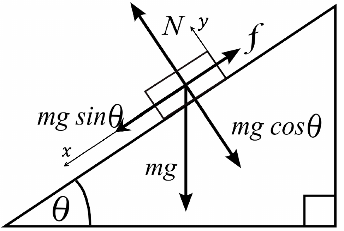
\includegraphics[width=0.9\linewidth]{scheme.png} 
			\caption{К выводу закона движения\\ по наклонной плоскости}
			\label{fig:subim1}
		\end{subfigure}
		\begin{subfigure}{0.5\textwidth}
			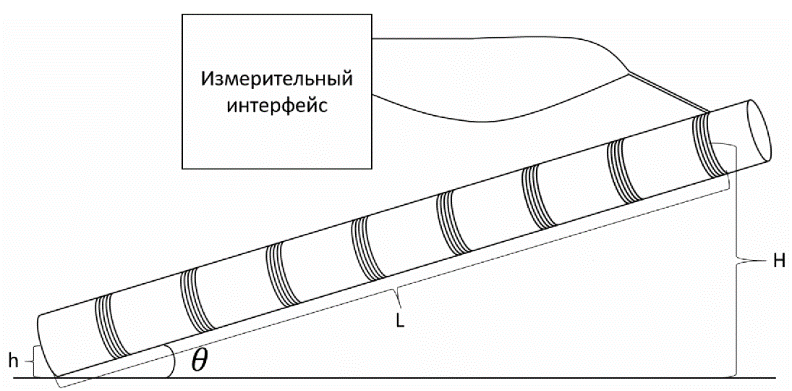
\includegraphics[width=0.9\linewidth]{tube.png}
			\caption{Экспериментальная установка}
			\label{fig:subim2}
		\end{subfigure}
	\end{figure}
	
	Запишем второй закон Ньютона в проекциях на наклонную плоскость $(ось Ox)$ и перпендикуляр к ней $(ось Oy)$, см. \ref{fig:subim1}:
	\begin{equation}
		Ox: ma = mg\sin{\theta} - f,
		\label{first}
	\end{equation}
	\begin{equation}
		Oy: \:\:\:\:\:\:\:\:\:N = mg\cos{\theta}.
		\label{second}
	\end{equation}
	
	Здесь $\theta$ — угол наклона плоскости к горизонту, $f$ — сила трения, $a$ — ускорение тела, $N$ — сила реакции опоры, $g$ — ускорение свободного падения.
	Сила трения $f$ состоит из сопротивления воздуха и силы трения о плоскость. Можно предположить, что основной вклад в
	силу трения вносит сухое трение, пропорциональное силе реакции опоры.
	Тогда $f$ = $\mu$ , где $\mu$ — коэффициент трения скольжения, зависящий только от свойств материалов.
		
	Решая систему \ref{first} и \ref{second}, получим выражение для ускорения:
	\begin{equation}
		a = g(\sin{\theta} - \mu\cos{\theta})
	\end{equation}
	
	Закон прямолинейного равноускоренного движения вдоль оси Ox, как известно, имеет вид:
	\begin{equation}
		x = v_{0}t + \frac{at^{2}}{2},
	\end{equation}
	где $x$ — координата тела, $v_0$ — начальная скорость (скорость в точке $x=0$).
	
	При приближении магнита к катушке поле вблизи катушки (а значит и его поток)
	сначала нарастает (по модулю), достигает максимума в средней точке, и затем, по мере удаления магнита, убывает до нуля. Исследуемый сигнал имеет два экстремума: последовательные максимум и минимум с прохождением через 0 (см \ref{fig:subim3}) Зависимость напряжения в цепи катушек от времени представляет собой набор пиков (см. \ref{fig:subim4})
	
	\begin{figure}[h]
		\begin{subfigure}{0.5\textwidth}
			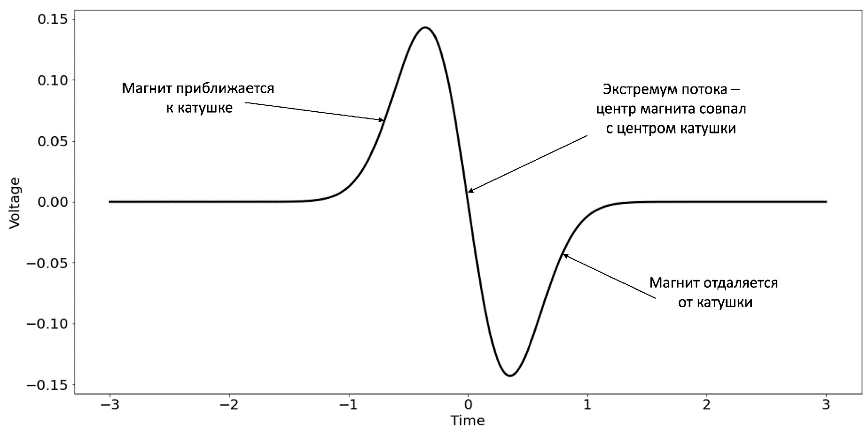
\includegraphics[width=0.9\linewidth]{once.png} 
			\caption{Зависимость напряжения от времени при пролёте магнита через одну катушку}
			\label{fig:subim3}
		\end{subfigure}
		\begin{subfigure}{0.5\textwidth}
			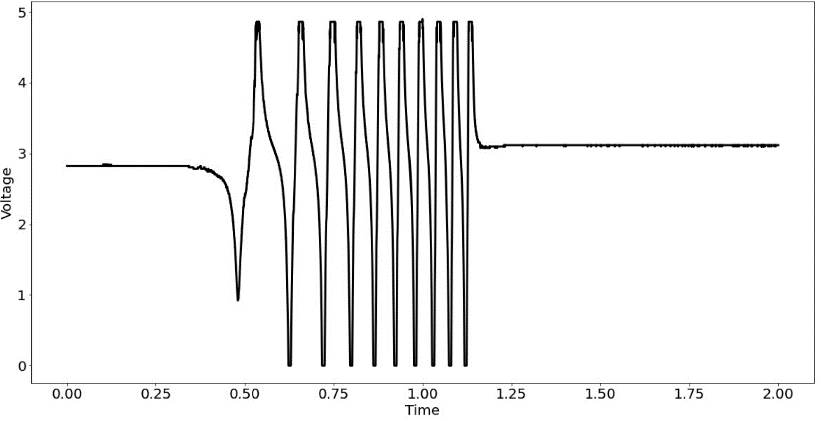
\includegraphics[width=0.9\linewidth]{multi.png}
			\caption{Пример сигнала при пролёте магнитом 10 катушек}
			\label{fig:subim4}
		\end{subfigure}
	\end{figure}
	
	Далее определяются параметры $v_0$ и $a$, при которых зависимость (\ref{fig:subim4}) наилучшим образом накладывается на экспериментальные точки.
	
	Используется численный \textit{метод наименьших квадратов}:
	\begin{equation}
		S = \sum_{n}\big(x_n - v_{0}t_{n} - \frac{at_{n}^{2}}{2}\big)^2 \rightarrow \min
	\end{equation}
	
	По результатам серии экспериментов при разных углах из пар значений {$a$, $\theta$} тем же методом наименьших квадратов для теоретической зависимости (\ref{fig:subim3}) определяются параметры ускорение свободного падения $g$ и коэффициент трения $\mu$.
	Для линеаризации зависимости (\ref{fig:subim3}) можно использовать, например, замену
	\begin{equation}
		a' = \frac{a}{\cos{\theta}}
	\end{equation}
	
	\begin{equation}
		\tau = \tg{\theta}
	\end{equation}
	
	Тогда
	\begin{equation}
		a' = g(\tau - \mu)
	\end{equation}
	
	\section{Оборудование и инструментальные погрешности}
	\textbf{Оборудование:} труба с намотанными катушками, фиксируемая на штативе; неодимовые магниты; линейка; блок регистрации сигнала (усилитель + микроконтроллер с АЦП), соединённый с компьютером.
	\begin{itemize}
		\item \textbf{Линейка}: $\Delta \text{лин} = \pm0.1$ см (по цене деления)
		\item \textbf{Весы}: $\Delta m = \pm{5}$ мг (маркировка производителя)
		\item \textbf{Угломер электронный}: $\Delta \varphi = \pm{0.1}$ град (маркировка производителя)
	\end{itemize}
	
	\newpage
	
	\section{Результаты измерений и обработка данных}
	
	\subsection{Характеристики системы:}
	
	$m = 3.589\pm 0,005$ г,\\
	
	\begin{table}[h]
		\centering
		\begin{tabular}{|c|c|c|c|c|c|c|c|c|c|c|}
			\hline
			N катушки & 1 & 2 & 3 & 4 & 5 & 6 & 7 & 8 & 9 & 10  \\
			\hline
			x, см & 0.0 & 10.2 & 20.1 & 30.1 & 40.1 & 50.1 & 60.1 & 70.1 & 80.2 & 90.0 \\
			\hline
		\end{tabular}
		\caption{Результаты измерений координат катушек.}
		\label{table:1}
	\end{table}
	
	\subsection{Измерения:}

	
	%\newpage
	
	\begin{table}[h]
		\centering
		\begin{tabular}[H]{|c|c|c|c|c|c|}
			\hline
			\textnumero & $\theta$, град & $a_{\min},\frac{\text{м}^2}{\text{с}^2}$ & $\sigma_{\min},\frac{\text{м}^2}{\text{с}^2}$ & $a_{\max},\frac{\text{м}^2}{\text{с}^2}$ & $\sigma_{\max},\frac{\text{м}^2}{\text{с}^2}$  \\
			\hline
			1 & 14.9 & 0.794 & 0.011 & 0.774 & 0.012 \\
			\hline
			2 & 14.9 & 0.771 & 0.013 & 0.752 & 0.012 \\
			\hline
			3 & 14.9 & 0.731 & 0.010 & 0.745 & 0.011 \\
			\hline
			4 & 25.1 & 2.507 & 0.011 & 2.489 & 0.007 \\
			\hline
			5 & 25.1 & 2.410 & 0.009 & 2.436 & 0.07 \\
			\hline
			6 & 25.1 & 2.422 & 0.013 & 2.380 & 0.018 \\
			\hline
			7 & 35.0 & 3.741 & 0.014 & 3.737 & 0.027 \\
			\hline
			8 & 35.0 & 3.834 & 0.015 & 3.778 & 0.025 \\
			\hline
			9 & 35.0 & 3.993 & 0.007 & 3.959 & 0.013 \\
			\hline
			10 & 45.8 & 6.241 & 0.041 & 6.192 & 0.039 \\
			\hline
			11 & 45.8 & 6.253 & 0.025 & 6.257 & 0.033 \\
			\hline
			12 & 45.8 & 6.232 & 0.049 & 6.223 & 0.037 \\
			\hline
			13 & 55.4 & 6.881 & 0.027 & 6.854 & 0.044 \\
			\hline
			14 & 55.4 & 6.836 & 0.049 & 6.941 & 0.028 \\
			\hline
			15 & 55.4 & 7.011 & 0.040 & 6.851 & 0.035 \\
			\hline
			16 & 65.0 & 8.117 & 0.057 & 8.173 & 0.070 \\
			\hline
			17 & 65.0 & 8.200 & 0.033 & 8.170 & 0.028 \\
			\hline
			18 & 65.0 & 8.220 & 0.050 & 8.127 & 0.038 \\
			\hline
		\end{tabular}
		\caption{Результаты измерений ускорений при различных углах.}
		\label{table:2}
	\end{table}
	
	\begin{table}[h]
		\centering
		\begin{tabular}[H]{|c|c|c|}
			\hline
			$\theta$, град & $a_{\text{ср}},\frac{\text{м}^2}{\text{с}^2}$ & $\sigma_{\text{ср}}$  \\
			\hline
			14.9 & 0.756 & 0.012 \\
			\hline
			25.1 & 2.440 & 0.011 \\
			\hline
			35.0 & 3.857 & 0.017 \\
			\hline
			45.8 & 6.233 & 0.037 \\
			\hline
			55.4 & 6.896 & 0.037 \\
			\hline
			65.0 & 8.168 & 0.046 \\
			\hline
		\end{tabular}
		\caption{Усредненные результаты измерений ускорений при различных углах.}
		\label{table:3}
	\end{table}
	
		Наконец, по результатам серии экспериментов при разных углах из пар значений {$a$, $\theta$} тем же \textit{методом наименьших квадратов} для теоретической зависимости (\ref{fig:subim3}) определим параметры ускорения свободного падения $g$ и коэффициент трения $\mu$:
	\begin{equation}
		\mu = 0.190 \pm 0.018; \:\:\: g = 9.689 \pm 0.330 \frac{\text{м}^2}{\text{c}}
	\end{equation}
	
	Ниже на Рис.\ref{graph} представлен график зависимости ускорения от угла наклона трубы
	\begin{figure}[h]
		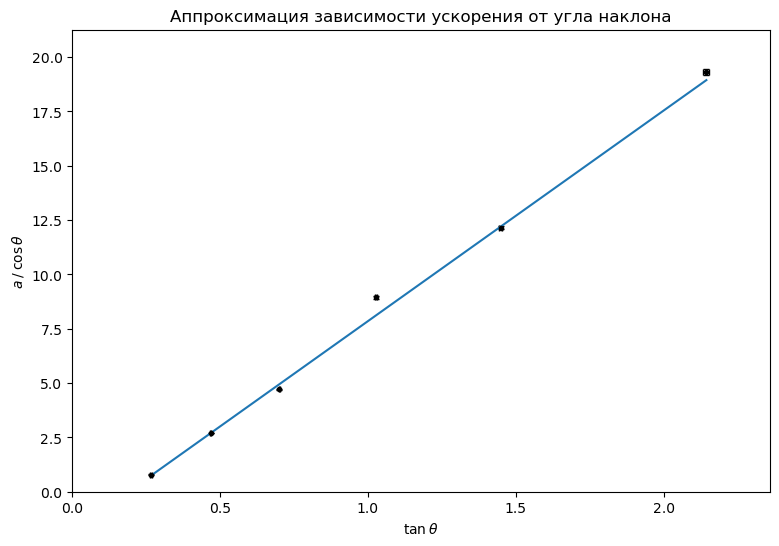
\includegraphics[width=0.9\textwidth]{graphic.png}
		\caption{Зависимость ускорения от угла наклона трубы}
		\label{graph}
	\end{figure}
	
	
	\section{Заключение}
	В ходе эксперимента получены величины ускорения свободного падения g и коэффициент трения скольжения $\mu$ трубы. Получилось, что ускорение свободного падения с точность до погрешности равна g = 9.69, что подтверждает применимость законов Ньютона на практике.
	
	
\end{document}
